We describe multiple equivalent constructions of a toric variety starting from the data
of a polytope $P$ subject to certain conditions. Each of 
the constructions will yield us a space $X_i(P)$ which will all be 
equivariantly diffeomorphic to each other as smooth manifolds. 


% Depending on the nature of the construction, $X_i(P)$ will either be 
% a projective toric variety or a toric symplectic manifold, and these 
% two classes of spaces can be identified with each other via the image 
% of their moment maps.

\subsection{Delzant polytopes}
Let $V$ be a real vector space of dimension $n$ and let $V_\Z$
be a lattice inside $V$. Given 
$N$ linear functionals $a_i \in V^*$ preserving $V_\Z$ and $N$ integers $\lambda_i$
the set \begin{align*}
P = \{ v \in V \mid a_i(v) + \lambda_i \geq 0 \text{ for all } i \}.
\end{align*} is called a \emph{rational polyhedron}. It is called 
a \emph{rational polytope} if it is bounded. We will assume that $P$ is a
rational polytope throughout this paper. A polytope $P$ has \emph{facets} \begin{align*}
F_i = \{ v \in P \mid a_i(v) + \lambda_i = 0 \}
\end{align*} and \emph{faces} which are intersections of facets. 
The \emph{vertices} of $P$ are the 0-dimensional faces of $P$ and 
the \emph{edges} of $P$ are the 1-dimensional faces of $P$.
We say $P$ is: \begin{itemize}
    \item \emph{simple} if exactly $n$ edges meet at each vertex
    \item \emph{smooth} if the edges meeting at each vertex form a basis for $V_\Z$
    \item \emph{Delzant} if $P$ is simple and smooth
\end{itemize}

\begin{example}
    The right triangle $P = \{ (x,y) \in \R^2 \mid x \geq 0, y \geq 0, x + y \leq 1 \}$ is a 
    Delzant polytope. The standard tetrahedron $P\subset\R^3$ is not Delzant because the
    top vertex is not simple.
\end{example}
We begin by stating the correspondence we are interested in.
\begin{theorem}\label{thm:delzant}
    [Delzant] There is a correspondence between Delzant polytopes up to $\GL(n,\Z)$ 
    and translation, and toric symplectic manifolds up to equivariant symplectomorphism.
\end{theorem}

\begin{theorem}
    There is a correspondence between Delzant polytopes up to $\GL(n,\Z)$
    and translation, and smooth projective toric varieties with a particular choice
    of very ample line bundle, up to equivariant isomorphism.
\end{theorem}

\subsection{Moment maps}
Let $(M,\omega)$ be a symplectic manifold. The nondegeneracy of $\omega$ allows us to
pair vector fields with 1-forms. We say that a vector field $X$ is \emph{Hamiltonian} if
the corresponding 1-form $\iota_X\omega = \omega(X,\cdot)$ is exact, in which case 
it is equal to $dH$ for some smooth function $H$. The function $H$ is called a
\emph{Hamiltonian} of $X$. 

Given a Lie group $G$ acting on $M$ by symplectomorphisms,
the Lie algebra $\mathfrak{g}$ acts on $M$ by symplectic vector fields.
This linearized action of $\mf g$ is given by the expression
\begin{align*}
    X_\zeta(m) = \frac{d}{dt}\Big|_{t=0} \exp(t\zeta)\cdot m
\end{align*} where we interpret the given expression via parallel transport along the flow of $\zeta$.

\begin{remark}
    In general, whenever we have a Lie group $G$ acting on a manifold $M$, we get a linearized
    action of $\mf g$ on $\Gamma(E)$ for any vector bundle $E$ over $M$. For the trivial 
    line bundle $E = M\times \R$ we have $\Gamma(E) = C^\infty(M)$ and the linearized action
    of $\mf g$ on $C^\infty(M)$ is given by the Lie derivative of 
    the function along the vector field.
\end{remark}

\begin{example}
    Consider $G = \SL(2,\C)$ acting on $\P^1$ by linear fractional transformations. Explicitly
    we have \begin{align*}
        \begin{pmatrix}
            a & b \\
            c & d
        \end{pmatrix} \cdot [z_0:z_1] = [az_0 + bz_1 : cz_0 + dz_1]
    \end{align*} The Lie algebra $\mf{sl}(2,\C)$ is generated by the matrices \begin{align*}
        E = \begin{pmatrix}
            0 & 1 \\
            0 & 0
        \end{pmatrix} \quad F = \begin{pmatrix}
            0 & 0 \\
            1 & 0
        \end{pmatrix} \quad H = \begin{pmatrix}
            1 & 0 \\
            0 & -1
        \end{pmatrix}
    \end{align*} Writing down the exponential, we find that \begin{align*}
        \exp(tE) = I + tE \quad \text{since } E^2 = 0
        \implies \exp(tE)\cdot [z_0:z_1] = [z_0 + tz_1 : z_1]
    \end{align*} On an affine chart, the action of $E$ is given by $z \mapsto z + t$ and
    we compute \begin{align*}
        \frac{d}{dt}\Big|_{t=0} z + t = 1 \implies X_E(z) = \frac{\partial}{\partial z}
    \end{align*} Similarly we compute \begin{align*}
        \exp(tH) = \begin{pmatrix}
            e^t & 0 \\
            0 & e^{-t}
        \end{pmatrix} \implies \exp(tH)\cdot [z_0:z_1] = [e^tz_0 : e^{-t}z_1]
    \end{align*} which looks like $z\mapsto e^{2t}z$ on an affine chart, which gives us
     \begin{align*}
        \frac{d}{dt}\Big|_{t=0} e^{2t}z = 2z \implies X_H(z) = 2z \frac{\partial}{\partial z}
    \end{align*} Finally we compute \begin{align*}
        \exp(tF) = 1 + tF \implies \exp(tF)\cdot [z_0:z_1] = [z_0 : z_1 + tz_0]
    \end{align*} On an affine chart this transformation looks like $z\mapsto z/(1+tz)$
    and we compute \begin{align*}
        \frac{d}{dt}\Big|_{t=0} \frac{z}{1+tz} = -z^2 \implies X_F(z) = -z^2\frac{\partial}{\partial z}
    \end{align*} In particular we get a map $\mf{sl}(2,\C) \to \Gamma(T\P^1)$ given by
    \begin{align*}
        E &\mapsto \frac{\partial}{\partial z} \\
        H &\mapsto 2z\frac{\partial}{\partial z} \\
        F &\mapsto -z^2\frac{\partial}{\partial z}
    \end{align*} which gives coordinates for the action of $\mf{sl}(2,\C)$ on $\Gamma(T\P^1)$.
    Recall that $T\P^1 \cong \cO(2)$ and $\dim \Gamma(T\P^1) = 3$. In particular, $\mf{sl}(2,\C)$
    acts on $\Gamma(T\P^1)$ by the standard representation. In general, this isomorphism can be thought of as 
    happening in degree $1$. This map extends to a graded isomorphism between the enveloping algebra $U(\mf{sl}(2,\C))$ and 
    the algebra of differential operators $\cD_{\text{hol}}(\P^1)$ on $\P^1$. This is a 
    shadow of the Beilinson-Bernstein localization theorem (see \cite{htt}).
\end{example}

Let $M$ be a symplectic manifold. We say that the action of $T$ on $M$ is \emph{weakly Hamiltonian} if for every $\zeta\in\mf t$ the corresponding vector field $X_\zeta$ is Hamiltonian,
i.e. $\iota_{X_\zeta}\omega = dH_\zeta$ for some smooth function $H_\zeta$. The $H_\zeta$
is determined only up to a constant, so choose the map $\mf g \to C^\infty(M)$ given by 
$\zeta \mapsto H_\zeta$ to be linear. If the map can be chosen to be equivariant with respect
to the adjoint action of $T$ on $\mf t$, then the action of $T$ is called \emph{Hamiltonian}.
In this case, there is a map $\mu : M \to \mf t^*$ called the \emph{moment map} defined by
\begin{align*}
    H_\zeta(m) := \langle \mu(m), \zeta \rangle
\end{align*}
If the action of $T$ is Hamiltonian, then the moment map is $T$-equivariant and unique up 
to the addition of a constant. In particular since $T$ is abelian, the adjoint action 
is trivial and the moment map $\mu : M \to \mf t^*$ is $T$-invariant. We are now prepared to state a foundational result in the classification of toric symplectic manifolds. For a 
complete reference, see \cite{mcduff-salamon}
\begin{theorem}\label{thm:ags}
    [Atiyah-Guillemin-Sternberg Convexity Theorem] Let $M$ be a compact connected symplectic manifold with a
    Hamiltonian $T$-action. Then the image of the moment map is a convex polytope 
    in $\mf t^*$ whose vertices are the image of the fixed points of the $T$-action.
\end{theorem}
We say $M$ is a \emph{toric symplectic manifold} in the sense of Theorem \ref{thm:delzant}
if $(M,\omega)$ is a compact connected symplectic manifold
with a effective (meaning no element of $T$ acts trivially) Hamiltonian $T$-action.


\subsection{Symplectic reduction}
We describe how to construct $M$ as the symplectic reduction of affine space $\C^N$ for 
a particular moment map. In particular, $M$ carries a natural symplectic form $\omega$ and 
a Hamiltonian $T$-action.
This section follows \cite{lsg}. 

Let $P$ be a Delzant polytope.
There are maps \begin{align*}
    \pi:\R^N&\to\R^n\\
    e_i &\mapsto a_i
\end{align*} and the induced map \begin{align*}
    \pi: \R^N/\Z^N\to\R^n/\Z^n 
\end{align*} of tori, which give rise to the following short exact sequences. \begin{align}\label{eq:ses1}
    1\to K \to \T^N \to \T^n \to 1
\end{align} \begin{align*}
    0\to k \to \R^N\to \R^n\to 0
\end{align*} The dual of the second sequence gives \begin{align*}
    0 \to (\R^n)^* \to (\R^N)^* \to k^* \to 0
\end{align*} and denote the map $i^* : (\R^N)^*\to k^*$. Now consider $\C^N$
with the standard symplectic form $\omega = \sum dz_i\wedge d\bar z_i$ and the 
standard Hamiltonian torus action \begin{align*}
    (e^{i\theta_1},\dots,e^{i\theta_N})\cdot(z_1,\dots,z_N) = (e^{i\theta_1}z_1,\dots,e^{i\theta_N}z_N)
\end{align*} and corresponding moment map \begin{align*}
    \phi:\C^N&\to(\R^N)^* \\
    \phi(z_1,\dots,z_N) &= -\pi(|z_1|^2,\dots,|z_N|^2) + (\lambda_1,\dots,\lambda_N)
\end{align*}
The subtorus $K$ acts on $\C^N$ via restriction and the restricted action is 
Hamiltonian. Moreover, the moment map for the action of $K$ is given by $i^*\circ\phi:M\to k^*$.

Let $Z = (i*^\circ \phi)^{-1}(0)$ be the zero level set of the moment map. The following 
claims are all justified in \cite{lsg}.

\begin{lemma}
    $Z$ is compact and $K$ freely acts on $Z$. 
\end{lemma}

The following theorem tells us that the orbit space $Z/K$ is a symplectic manifold.

\begin{theorem}{\label{thm:reduction}}
    [Marsden-Weinstein-Meyer] Let $G$ be a compact group and let $(M,\omega)$ be a symplectic manifold with a
    Hamiltonian $G$-action. Let $i:\mu^{-1}(0)\to M$ be the inclusion of the zero level set of the moment map.
    Assume $G$ acts freely on $\mu^{-1}(0)$. Then \begin{itemize}
        \item the orbit space $M_{\text{red}} = \mu^{-1}(0)/G$ is a smooth manifold
        \item $\pi:\mu^{-1}(0)\to M_{\text{red}}$ is a principal $G$-bundle
        \item there is a unique symplectic form $\omega_{\text{red}}$ on $M_{\text{red}}$ such that $\pi^*\omega_{\text{red}} = i^*\omega$
    \end{itemize}
\end{theorem}
Symplectic reduction realizes one direction of Delzant's correspondence.
\begin{proposition}
    The reduced space $X_1(P) := Z/K$ is a toric symplectic manifold with moment map image $P$.
\end{proposition}

\subsection{Projective GIT}
Let $P$ be a Delzant polytope. Complexifying (\ref{eq:ses1}), we get \begin{align*}
    1\to K_\C \to T_\C^N \to T_\C^n \to 1 
\end{align*} Let $F_i$ denote the facets of $\Delta$ and for any $z = (z_1,\dots,z_N)\in\C^n$ let $F_z := \cap_{z_i = 0}F_i$.
Consider the set \begin{align*}
    U = \{z\in\C^n: F_z \neq \emptyset\}
\end{align*} Then the quotient $X_2(P) = U/K_\C$ is a manifold with an action of $T_\C^N/K_\C = T_\C^n$. It is a smooth projective toric variety because it is a projective GIT quotient, as we will explain with the following theorem of Kempf-Ness.

\begin{remark}
    There is a surjective map from $X^{\text{ss}}$ to $X//G$. Two points in $X^{\text{ss}}$
    lie in the same fiber of this map if and only if the closures of their 
    $G$-orbits intersect. In this case, the $K_\C$ orbits are closed. See \cite{proudfoot} for more details.
\end{remark}
\begin{proposition}
    Let $M\subset \C\P^n$ be a smooth projective toric variety embedded by a line bundle.
    Then $M$ is equivariantly symplectomorphic to a toric symplectic manifold.
\end{proposition}
\begin{proof}
$\C\P^n$ carries a natural symplectic form $\omega$ 
called the Fubini-Study form. Any smooth projective toric variety $M$ embedded
in projective space carries a symplectic form $\omega$ induced by pulling 
back the Fubini-Study form. Moreover, the action of $T$ on $M$
 is Hamiltonian with respect to $\omega$.
\end{proof}

Conversely, given a toric symplectic manifold $(M,\omega)$, we can associate a 
smooth projective toric variety to the moment polytope $\mu(M)$ which will be
equivariantly symplectomorphic to $M$.
\subsection{Kempf-Ness theorem}
The Kempf-Ness theorem provides a connection between algebraic geometry and symplectic geometry. 
Recall that if $K$ is a real compact group, then its complexification $G := K_\C$ is a 
complex Lie group which contains $K$ and $\mf g = \mf k \oplus i\mf k$ is the complexification of $\mf k$. See \cite{hoskins} for more details about the following theorems.

\begin{theorem}
    Complexification defines a bijection between the isomorphism
    classes of compact real Lie groups and complex reductive groups.
\end{theorem}
The following theorem of Kempf-Ness establishes a relationship between the reduction of a Hamiltonian system by the real group $K$ and the corresponding projective GIT quotient by the complex group $G$.
\begin{theorem}{\label{thm:kempf-ness}}
    [Kempf-Ness] 
    Let $G$ be a complex reductive group acting on a smooth complex projective variety 
    $X\subset \P^n$. Let $K$ be a maximal compact subgroup of $G$ and suppose $K$ 
    is connected and acts on $X$ Hamiltonianly. Let $\mu:X\to\mf k^*$ be the moment map. 
    Then the inclusion $\mu^{-1}(0)\to X$ induces a homeomorphism \begin{align*}
        \mu^{-1}(0)/K \to X//G
    \end{align*}
\end{theorem}

\begin{remark}
This theorem is fundamental in moduli problems, where spaces of equivalence classes of geometric objects (like vector bundles, sheaves, or varieties) can be constructed as quotients.
It is widely used in understanding spaces like the moduli of vector bundles, the geometry of flag varieties, and moment polytope theory.
\end{remark}

\subsection{Fans and abstract toric varieties}

Let \( T \) be an \( n \)-dimensional torus with character group \( M \),
 and let \( N = \operatorname{Hom}_{\mathbb{Z}}(M, \mathbb{Z}) \) be
  the dual lattice, with pairing denoted \( \langle , \rangle \). Recall that Theorem \ref{thm:delzant} gives a correspondence between Delzant polytopes 
and smooth projective toric varieties equipped with a very ample line bundle.
Forgetting the embedding, we pass to the abstract toric variety, whose combinatorics is encoded in the data of a fan.

\begin{definition}
    A \emph{fan} $\Sigma$ in a real vector space $N$ is a collection of cones
    $\sigma$ such that \begin{itemize}
        \item $\sigma$ is a strongly convex polyhedral cone
        \item if $\sigma\in\Sigma$ and $\tau$ is a face of $\sigma$, then $\tau\in\Sigma$
        \item the intersection of any two cones in $\Sigma$ is a face of each
    \end{itemize}
\end{definition}

Given a Delzant polytope $P$, there is a fan $\Sigma_P$ in $N_\R$ obtained by taking 
normal directions to the facets of $P$. The fan $\Sigma_P$ is called the \emph{normal fan} of $P$
and it is a combinatorial object which encodes an equivariant atlas of charts for the toric variety $X(P)$.

\begin{definition}
    A fan $\Sigma$ is \emph{complete} if the union of the cones in $\Sigma$ is all of $N_\R$.
    A fan $\Sigma$ is \emph{nonsingular} if for each $k$-dimensional cone $\sigma\in\Sigma$,
    there exist $k$ lattice vectors $v_1,\dots,v_k$ such that $\{v_1,\dots,v_k\}$ generate $\sigma$
    and $v_1,\dots,v_k$ can be extended to a basis of $N$.
    A fan $\Sigma$ is \emph{projective} if there is a rational polytope $P$ such that $\Sigma$ is the normal fan of $P$.
\end{definition}

As the geometric language suggests, the toric variety $X(\Sigma)$ corresponding to a fan $\Sigma$ is complete if and only if the fan is complete, and $X(\Sigma)$ is smooth if and only if the fan is nonsingular. See \cite{cls} for more details. 

\begin{example}
    Consider the unit right triangle with corresponding normal fan
    \begin{figure}[H]
        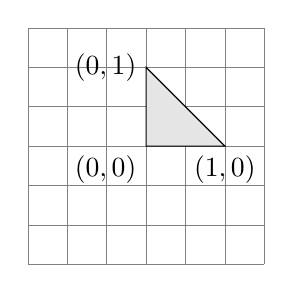
\begin{tikzpicture}[scale=0.5]
            \draw[step=1cm,gray,very thin] (-3,-3) grid (3,3);
            \filldraw[fill=gray!20, draw=black] (0,0) -- (2,0) -- (0,2) -- cycle;
            \node at (0,0) [below left] {$(0,0)$};
            \node at (2,0) [below] {$(1,0)$};
            \node at (0,2) [left] {$(0,1)$};
        \end{tikzpicture}
        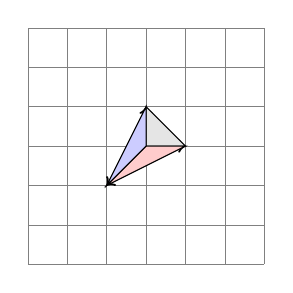
\begin{tikzpicture}[scale=0.5]
            \draw[step=1cm,gray,very thin] (-3,-3) grid (3,3);
            \draw[thick,->] (0,0) -- (1,0);
            \draw[thick,->] (0,0) -- (0,1);
            \draw[thick,->] (0,0) -- (-1,-1);
            % fill in the upper right quadrant
            \filldraw[fill=gray!20, draw=black] (0,0) -- (1,0) -- (0,1) -- cycle;
            % fill in the region from pi/2 to 5pi/4 
            \filldraw[fill=red!20, draw=black] (0,0) -- (-1,-1) -- (1,0) -- cycle;
            % fill in the region from 5pi/4 to 3pi/2
            \filldraw[fill=blue!20, draw=black] (0,0) -- (-1,-1) -- (0,1) -- cycle;
        \end{tikzpicture}
        \caption{Polytope and normal fan for $\C\P^2$}
    \end{figure}
    Note that the fan has three 2-dimensional cones which are filled in.
    These cones represent the three standard coordinate charts of $\P^2$ given by
    $x_i \neq 0$ for $i = 0,1,2$. The isosceles right triangle with
    side lenghth $a$ corresponds to the $a$-th Veronese 
    embedding of $\P^2$.
\end{example}
Fans are more friendly objects for algebraic geometers and 
one can read further about them in \cite{cls}. The data of a fan,
and in particular the primitive edge vectors (defined as the generators of the rays of the fan),
will prove important in our discussion on equivariant cohomology.

\subsection{Cone-orbit correspondence}
Let $T$ be an $n$-dimensional torus with character group $M$. Let $N = \Hom(M,\Z)$ be the
dual lattice, their pairing is denoted by $\langle \cdot,\cdot\rangle$. Let $X = X(\Sigma)$ be a smooth complete toric variety, which are in bijection with complete nonsingular fans $\Sigma$ in $N_\R$.

For any convex cone $\sigma \subset N_\R$, the \emph{dual cone} in $M_\R$ is \begin{align*}
	\sigma^\vee = \{u\in M_\R \mid \langle u,v\rangle \geq 0 \text{ for all } v\in \sigma\}.
\end{align*} By intersecting with the lattice, we obtain a semigroup $\sigma^\vee \cap M$
with corresponding semigroup algebra $\C[\sigma^\vee \cap M]$. The toric variety $X$
is covered by $T$-invariant open affine sets \begin{align*}
	U_\sigma = \Spec \C[\sigma^\vee \cap M]
\end{align*} The affine charts corresponding to the top-dimensional cones of $\Sigma$
are enough to cover $X$, and the intersection of cones corresponds to the intersection of
affine charts.

Each cone $\tau$ of the fan also defines a torus-invariant subvariety $V(\tau)$ of $X$ of codimension $\dim \tau$.
On open affines, the subvariety looks like \begin{align*}
	V(\tau) \cap U_\sigma = \Spec \C[\tau^{\perp} \cap \sigma^\vee \cap M] \hookrightarrow \Spec \C[\sigma^\vee \cap M]
\end{align*} and so elements of the dual lattice $N$ can be thought of as rational functions on $X$.


